% Included from both -slides and -handout versions.
\documentclass[pdftex]{beamer} % used to trigger beamer mode in Emacs,
                               % normally commented out.

\usetheme{metropolis}

\usepackage[english]{babel}
\usepackage[latin1]{inputenc}
\usepackage{graphicx}
\usepackage{times}
\usepackage[T1]{fontenc}
\usepackage{fancyvrb}
\usepackage{listings}
\begin{document}
\lstset{language=C, escapeinside={(*@}{@*)}, numbers=left,
  basicstyle=\tiny, showspaces=false, showtabs=false}

\title{Introduction to Operating Systems}
\subtitle{Through tracing, analysis, and experimentation}
%\institute{University of Cambridge}
\author{George V. Neville-Neil}
%\author{Dr Robert N. M. Watson}
\date{1 August 2016}

\begin{frame}
  \titlepage
\end{frame}

\section{Communcation}
\label{sec:communication}

\section{Inter-Process Communication}
\label{sec:ipc}

\begin{frame}
  \frametitle{Goals of IPC}
  \begin{itemize}
  \item Data Sharing
  \item Signaling events
  \item Control of multiple processes
  \end{itemize}
\end{frame}

\begin{frame}
  \frametitle{Mechanisms}
  \begin{itemize}
  \item Shared files
  \item Semaphores and Mutexes
  \item Signals
  \item Sockets
  \end{itemize}
\end{frame}

\begin{frame}
  \frametitle{History}
  \begin{itemize}
  \item 
  \item 
  \item 
  \end{itemize}
\end{frame}

\begin{frame}
  \frametitle{Relationship to Networking}
  \begin{itemize}
  \item Extension of mechanisms across machines
  \item Everything is a byte stream
  \item No record boundaries
  \item File like API
  \end{itemize}
\end{frame}

\begin{frame}
  \frametitle{Signals}
  \begin{itemize}
  \item Based on hardware interrupt model
  \item Not useful for data transfer
  \item Catch and process
  \end{itemize}
\end{frame}

\begin{frame}
  \frametitle{Signal Handling}
  \begin{itemize}
  \item Source raises a signal
  \item destination catches the signal 
  \item Uncaught signals cause a program to exit
  \end{itemize}
\end{frame}

\begin{frame}[fragile]
  \frametitle{Available Signals}
\resizebox{1.0\textwidth}{!}{%
  \begin{tabular}{l|l|l|l}
  Name & Meaning & Name & Meaning \\
  \hline
    SIGHUP & line hangup & SIGURG & urgent condition present on  socket \\
    SIGINT & interrupt program & SIGSTOP & stop (cannot be caught or ignored) \\
    SIGQUIT & quit program & SIGTSTP & stop signal generated from  keyboard \\
    SIGILL & illegal instruction & SIGCONT & continue after stop \\
    SIGTRAP & trace trap & SIGCHLD & child status has changed \\
    SIGABRT & abort program & SIGTTIN & background read attempted from control terminal \\
    SIGEMT & emulate instruction executed &  SIGTTOU & background write attempted to control terminal \\
    SIGFPE & floating-point exception & SIGIO & I/O is possible on	a descriptor \\
    SIGKILL & kill program & SIGXCPU & cpu time limit exceeded \\
    SIGBUS & bus error & SIGXFSZ & file size limit exceeded \\
    SIGSEGV & segmentation violation & SIGVTALRM & virtual time alarm \\
    SIGSYS & non-existent system call invoked & SIGPROF & profiling timer alarm \\
    SIGPIPE & write on a pipe with no reader & SIGWINCH & Window size change \\
    SIGALRM & eal-time timer expired & SIGINFO & status request from keyboard \\
    SIGTERM & software termination signal & SIGUSR1 & User defined signal 1 \\
    & & SIGUSR2 & User defined signal 2 \\
    & & SIGTHR & thread interrupt \\
    & & SIGLIBRT & real-time library interrupt
  \end{tabular}
}
\end{frame}

\begin{frame}[fragile]
  \frametitle{Pipes}
  \begin{itemize}
  \item Easliest bulk data IPC
  \item Key innovation of UNIX systems
  \item Depends on file descriptors
  \item \emph{STDIN} \emph{STDOUT} \emph{STDERR}
 \end{itemize}
\end{frame}

\begin{frame}
  \frametitle{Pipe Implementation}
  \begin{itemize}
  \item 
  \item 
  \item 
  \end{itemize}
\end{frame}

\section{Internetworked Communication}
\label{sec:internet}

\begin{frame}
  \frametitle{Networking and FreeBSD}
  \begin{itemize}
  \item Everyone's TCP/IP Stack
  \item IPv4, IPv6, UDP, TCP, SCTP
  \item Various drivers
  \item Multiple firewalls
  \end{itemize}
\end{frame}

\begin{frame}
  \frametitle{Networking: The ISO Model}
  \begin{itemize}
  \item Canonical description of network protocols
  \item Each protocols are layered
  \item Seven layers in all
  \item Beware Van Jacobsen's warning!
  \end{itemize}
\end{frame}

\begin{frame}
  \frametitle{Networking and Layering}
\centering
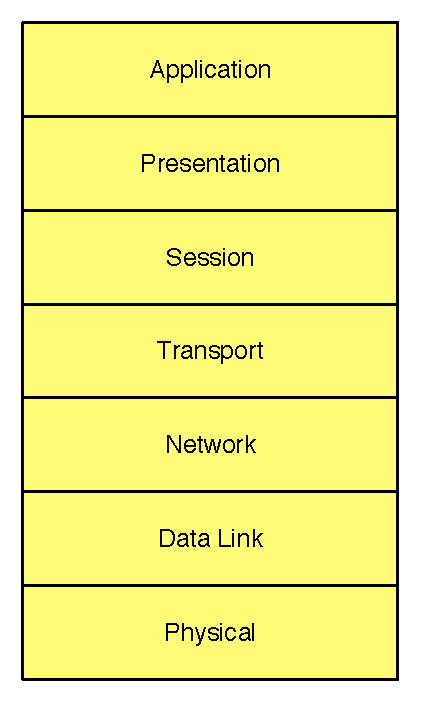
\includegraphics[width=0.4\textwidth]{../../figures/ISO-layers.pdf}
\end{frame}

\begin{frame}
  \frametitle{Networking and Layering}
\centering
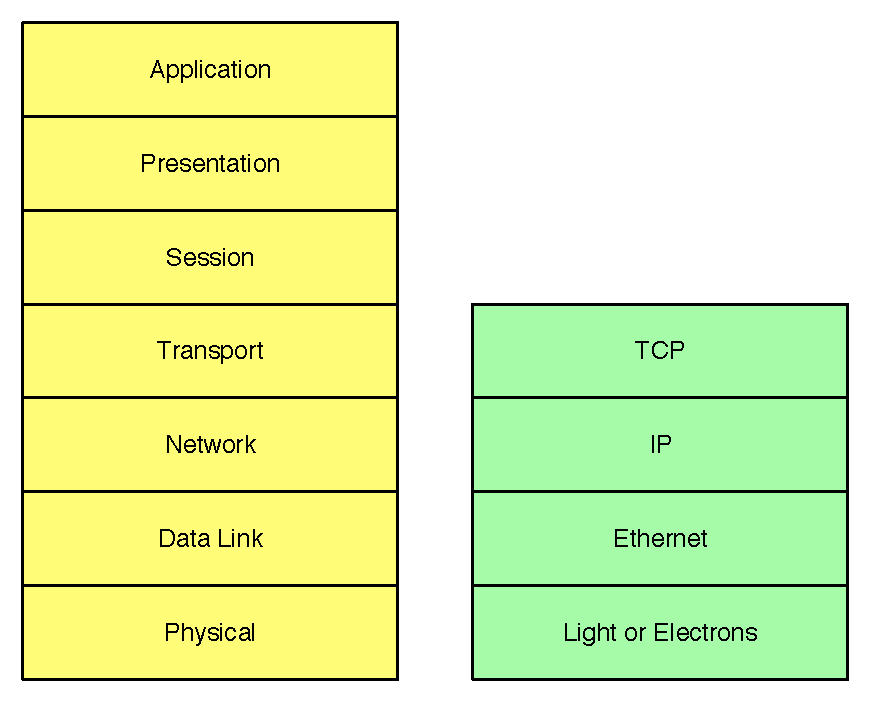
\includegraphics[width=0.7\textwidth]{../../figures/ISO-layers-mapped.pdf}
\end{frame}

\begin{frame}
  \frametitle{Networking and Layering}
\centering
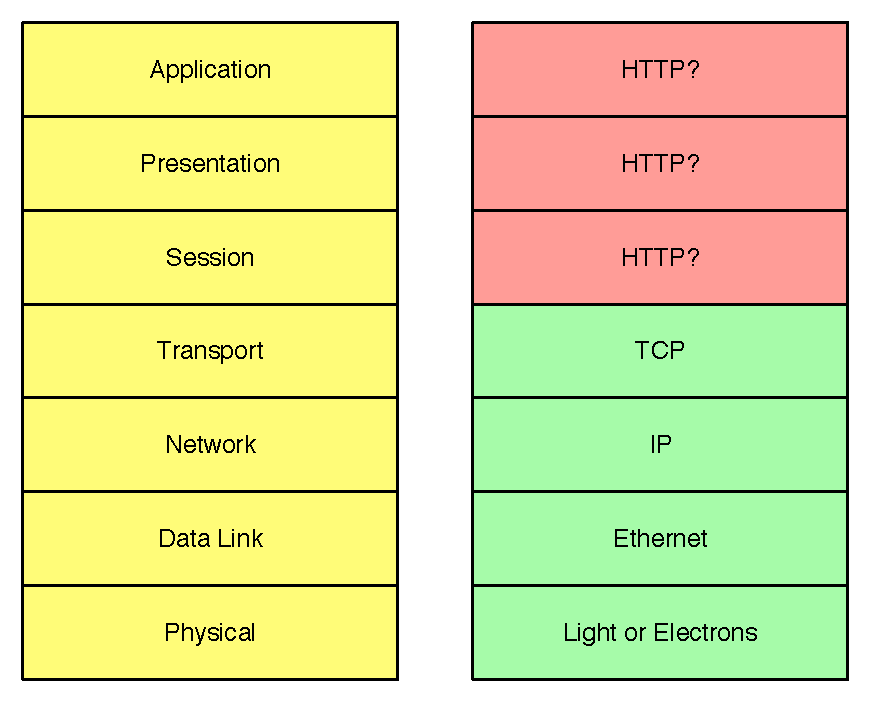
\includegraphics[width=0.8\textwidth]{../../figures/ISO-layers-http.pdf}
\end{frame}

\begin{frame}
  \frametitle{The User Program View}
  \begin{itemize}
  \item User programs use sockets
  \item Network programs follow UNIX model
  \item Flexible interfaces for different protocols
  \end{itemize}
\end{frame}

\begin{frame}
  \frametitle{Sockets}
  \begin{itemize}
  \item Main programmer interface to networking
  \item Generic API
  \item Attempts to support read/write semantics
  \end{itemize}
\end{frame}

\begin{frame}
  \frametitle{Network Stack Overview}
\centering
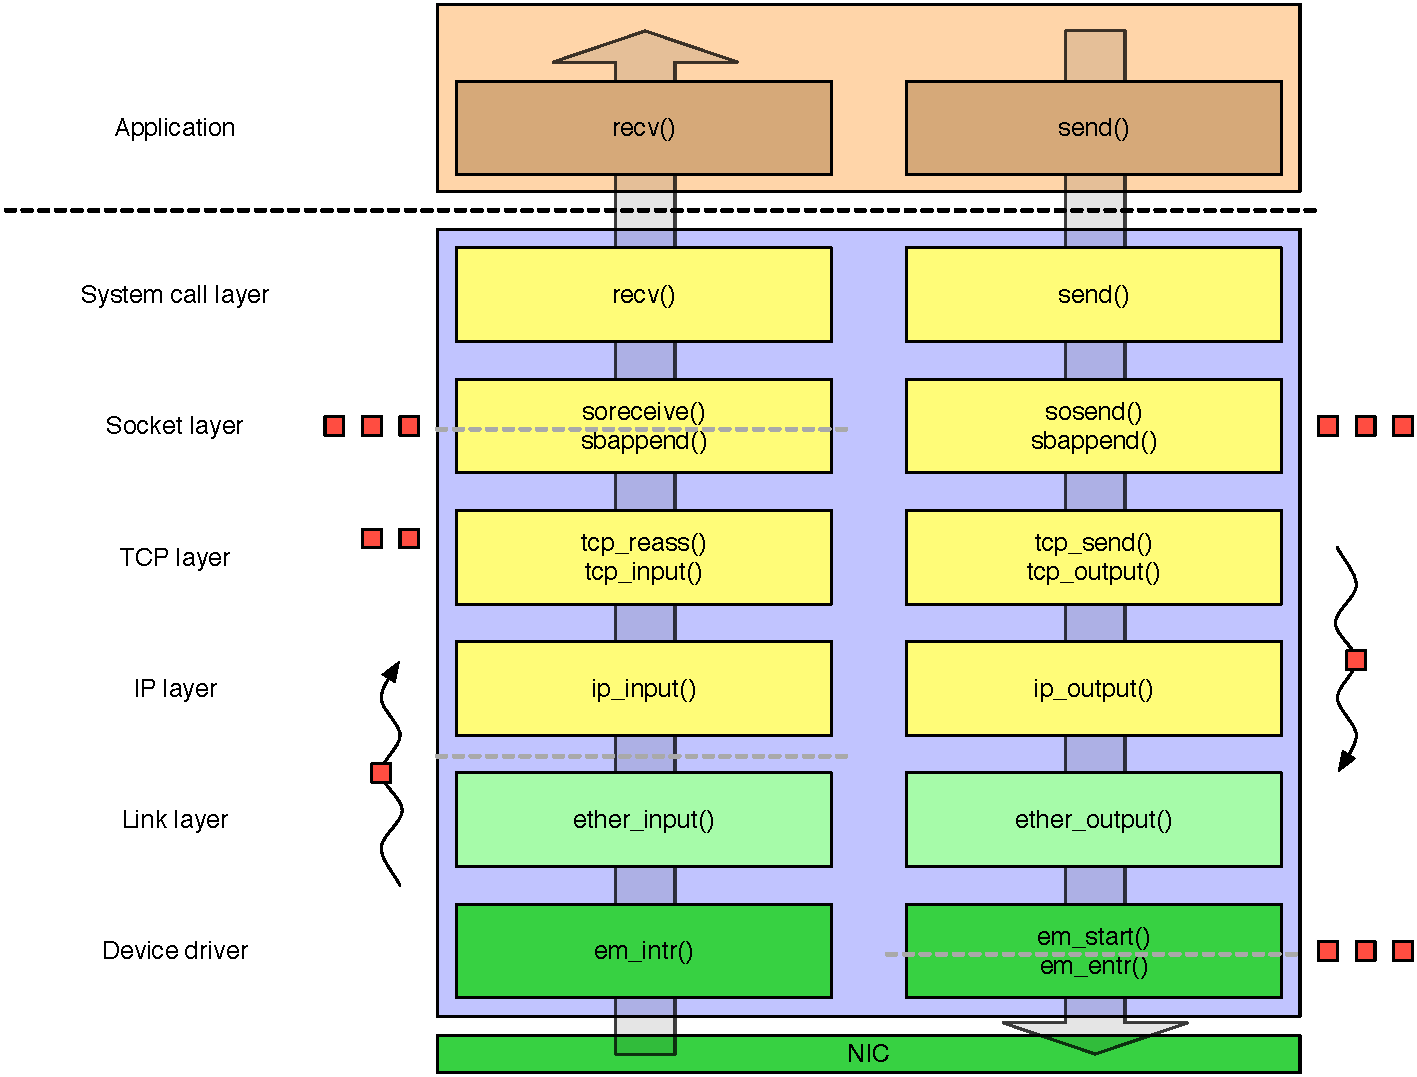
\includegraphics[width=0.8\textwidth]{../../figures/network-in-out.pdf}
\end{frame}

\begin{frame}[fragile]
  \frametitle{UDP}
  \begin{itemize}
  \item Simplest transport protocol
  \item No states to maintain
  \item Data is sent immediately
  \item Supports multicast
  \item Only probes are \verb+send+ and \verb+receive+
  \end{itemize}
\end{frame}

\begin{frame}
  \frametitle{TCP}
  \begin{itemize}
  \item Transmission Control Protocol
  \item Stream based
  \item In order delivery
  \item Maintains the illusion of a byte stream
  \end{itemize}
\end{frame}

\begin{frame}[fragile]
  \frametitle{TCP State Machine}
  \begin{itemize}
\centering
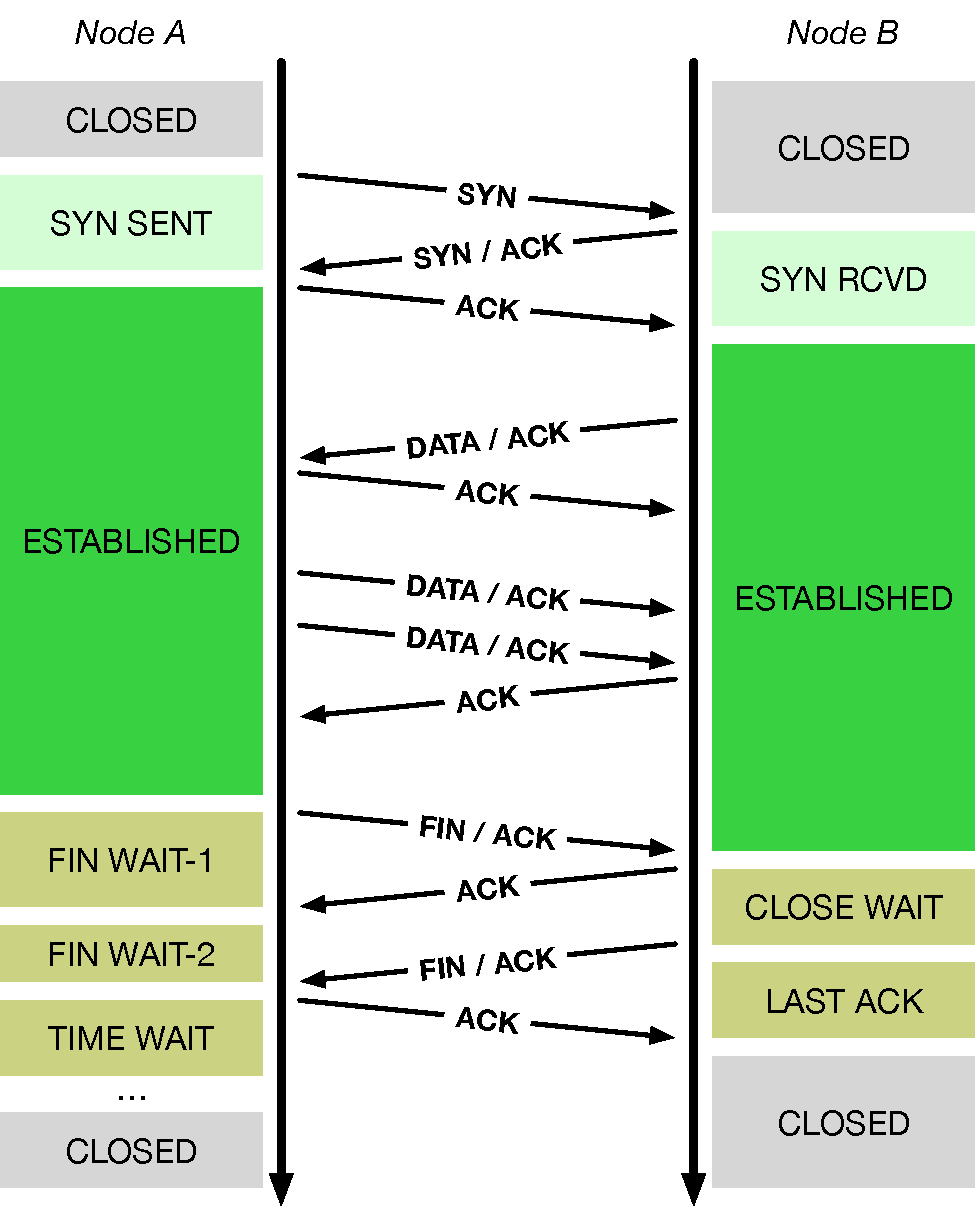
\includegraphics[width=0.6\textwidth]{../../figures/tcp-timeline.pdf}
  \end{itemize}
\end{frame}

\end{document}

%%% Local Variables:
%%% mode: latex
%%% TeX-master: "lecture3-communication"
%%% End:
